\documentclass[a4paper,11pt]{article}

\usepackage[english]{babel}
\usepackage{mathtools,amsthm,amssymb,amsmath}
\usepackage{a4wide}

\usepackage{fouriernc}
\usepackage{hyperref}
\usepackage[capitalize]{cleveref}


\usepackage{minted}
\setminted[python]{linenos=true}
\setminted[python]{frame=lines}
\setminted[R]{linenos=true}
\setminted[R]{frame=lines}


\usepackage{pythontex}
\setpythontexfv[]{numbers=left, frame=lines, label=\fbox{Python Code}, xleftmargin=5mm,framesep=2mm,fontsize=\small} %,samepage}
\restartpythontexsession{\thefigure}


\newcommand{\N}{\mathbb{N}}
\newcommand{\R}{\mathbb{R}}
\newcommand{\Z}{\mathbb{Z}}
\DeclareMathOperator*{\argmin}{arg\,min}

\newcommand{\abs}[1]{\left\vert#1\right\vert}
\newcommand{\given}{\,\middle|\,}
\newcommand{\Bern}[1]{\mathrm{Bern}(#1)}
\newcommand{\Bin}[1]{\mathrm{Bin}(#1)}
\newcommand{\Exp}[1]{\mathrm{Exp}(#1)}
\newcommand{\FS}[1]{\mathrm{FS}(#1)}
\newcommand{\Geo}[1]{\mathrm{Geo}(#1)}
\newcommand{\Norm}[1]{\mathrm{Norm}(#1)}
\newcommand{\Pois}[1]{\mathrm{Pois}(#1)}
\newcommand{\Unif}[1]{\mathrm{Unif}(#1)}
\renewcommand{\P}[1]{\,\mathsf{P}\left\{#1\right\}}
\newcommand{\E}[1]{\,\mathsf{E}\left[#1\right]}
\newcommand{\EE}[2]{\,\mathsf{E}_{#1}\left[#2\right]}
\newcommand{\V}[1]{\,\mathsf{V}\left[#1\right]}
\newcommand{\cov}[1]{\,\mathsf{Cov}\left[#1\right]}
\renewcommand{\d}[1]{\,\textrm{d}#1}
\newcommand{\1}[1]{\,I_{#1}} % indicator

\author{Claire Gun (s123456) and Clark Rifle (s654321)}
\date{\today}
\title{Prob dist., assignment 1\\
  2020-2021
  }
\begin{document}

\maketitle

Just to help you, read also the \verb|newcommands| above. Using such commands can make your life considerably easier.

\section{Exercise/question/problem 1}

In our understading, taking the product of two numbers comes down to repeating taking the sum of couple of times.

\section{Problem 2}

When we run the simulation, see the code and parameters below, we get the answer 50

\begin{minted}[]{python}
a = 10
b = 5
print(a*b)
\end{minted}


\begin{minted}[]{R}
a <- 5
b <- 10
b*a
\end{minted}

\section{Exercise/question/problem 3}

The graph is like this (check on \texttt{overleaf} (see the web), how to include graphs in \LaTeX).


\section{A minimal working example (MWE) for making plots}
\label{sec:minim-work-example}

If you like to keep code (to later check how you made things) and text in one file, you might like to use pythontex. To understand how this part works, you should read the documentation of pythontex. (I find it very practical.)  BTW, it also seems to work with R, but I havent't tested it. Anyway, here is a MWE. If you don't want to use pythontex, just remove this part of the source in the latex file.

\begin{figure}
\centering
\begin{pycode}
import numpy as np
from scipy.stats import uniform
import matplotlib.pyplot as plt

np.random.seed(3)


def superposition(F, N, num_visits):
    X = F.rvs((N, num_visits))
    A = X.cumsum(axis=1)
    A = np.sort(A.flatten())
    X = A[1:] - A[:-1]
    return X


fig, (ax1, ax2) = plt.subplots(1, 2, figsize=(5, 2))
plt.rcParams.update({"text.usetex": True})
plt.xlim(0)

F = uniform(loc=5.5, scale=1)  # distribution of interarrival times

N, v = 12, 100  # Num patients, num visits
labda = N / 6
X = superposition(F, N, v)
bins = np.linspace(0, 3 / labda, 50)
ax1.set_xlim([0, 3 / labda])
ax1.set_title(r'N=12, visits = 100')
ax1.hist(X, bins=bins, density=True)
exp_dens = labda * np.exp(-labda * bins)
ax1.plot(bins, exp_dens, color="black")

N, v = 120, 12  # Num patients, num visits
labda = N / 6
X = superposition(F, N, v)
bins = np.linspace(0, 3 / labda, 50)
ax2.set_xlim([0, 3 / labda])
ax2.hist(X, bins=bins, density=True)
exp_dens = labda * np.exp(-labda * bins)
ax2.set_title(r"N=120, visits = 12")
ax2.plot(bins, exp_dens, color="black")
plt.savefig("figures/poisson-exp-dist3.pdf", bbox_inches\textit='tight')
\end{pycode}
\IfFileExists{figures/poisson-exp-dist3.pdf}{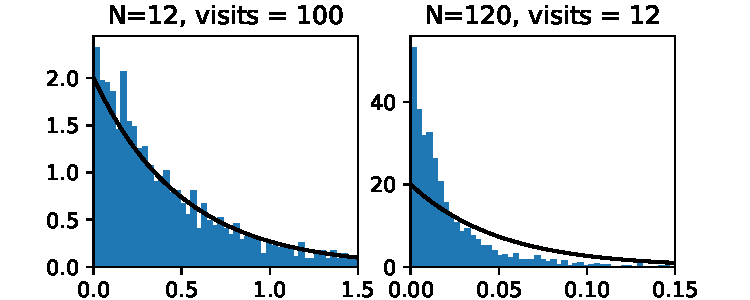
\includegraphics{figures/poisson-exp-dist3.pdf}}{}
\caption{The interarrival times for the case with $N=12$ patients and $100$ visits versus $N=120$ and $12$ visits.}
\label{fig:expdist3}
\end{figure}


\end{document}
